\chapter{Einleitung}

\section{Was ist der ewm-sim?}
In der vierten industriellen Revolution verändert sich auch der Arbeitsalltag in Lagerhallen. Mobile Roboter finden verstärkt Einsatz, um die Arbeiter zu unterstützen. Das Projekt \ac{EWM} Cloud Robotics der SAP hat das Ziel, ein Roboternetzwerk auf Basis von Google Cloud Robotics an ein SAP \ac{EWM}-System anzubinden. Zu Demonstrationszwecken wird eine Simlationsumgebung erstellt, in der ein virtuelles Warenlager präsentiert werden, in dem Roboter beispielhafte Aufträge bearbeiten. Um nun zu vermeiden, dass ein vollständiges \ac{EWM}-System für solch eine Simulation deployed werden muss, wurde \enquote{ewm-sim} eingeführt. Er stellt einen kleinen Web-Server dar, welcher die Schnittstelle, über die die Roboter ihre Aufträge vom \ac{EWM}-System erhalten, detailgetreu nachbildet.

\section{Kritikpunkte der ursprünglichen Implementierung}
Wie bereits erwähnt, soll der ewm-sim die Schnittstelle eines \ac{EWM}-Systems nachbilden. Hierbei handelt es sich um einen OData-Service. Für die Implementierung wurde hier auf den bestehenden MockServer von SAPUI5 gesetzt. Dieser ist jedoch zur Frontend- und nicht zur Backend-Entwicklung vorgesehen. Leider bringt er das Problem mit sich, dass er sich nur innerhalb einer SAPUI5-App verwenden lässt, welche wiederum in einem Browser läuft. In der \autoref{fig:ewm-sim-v1} ist der Aufbau des bisherigen ewm-sim veranschaulicht. Er stellt eine Art gekapseltes System dar. Die Anfragen, die gegen den nach außen hin geöffneten WebServer geschickt werden, landen über den WebSocket Server bei einer headless Instanz von Google Chrome, in welchem wiederum die SAPUI5-App ausgeführt wird. Diese ist mit dem SAPUI5 Mockserver verknüpft, welcher die Daten, die er bereitstellen soll, aus \code{\ac{JSON}}-Dateien einliest.

Wie gut zu erkennen ist, bringt diese Implementierung einen großen Overhead und mögliche Fehlerquellen mit sich. Ziel des in dieser Praxisarbeit behandelten Projekts soll es sein, das Konzept des ewm-sim zu optimieren und diesen neu zu implementieren.

\begin{figure}
    \centering
    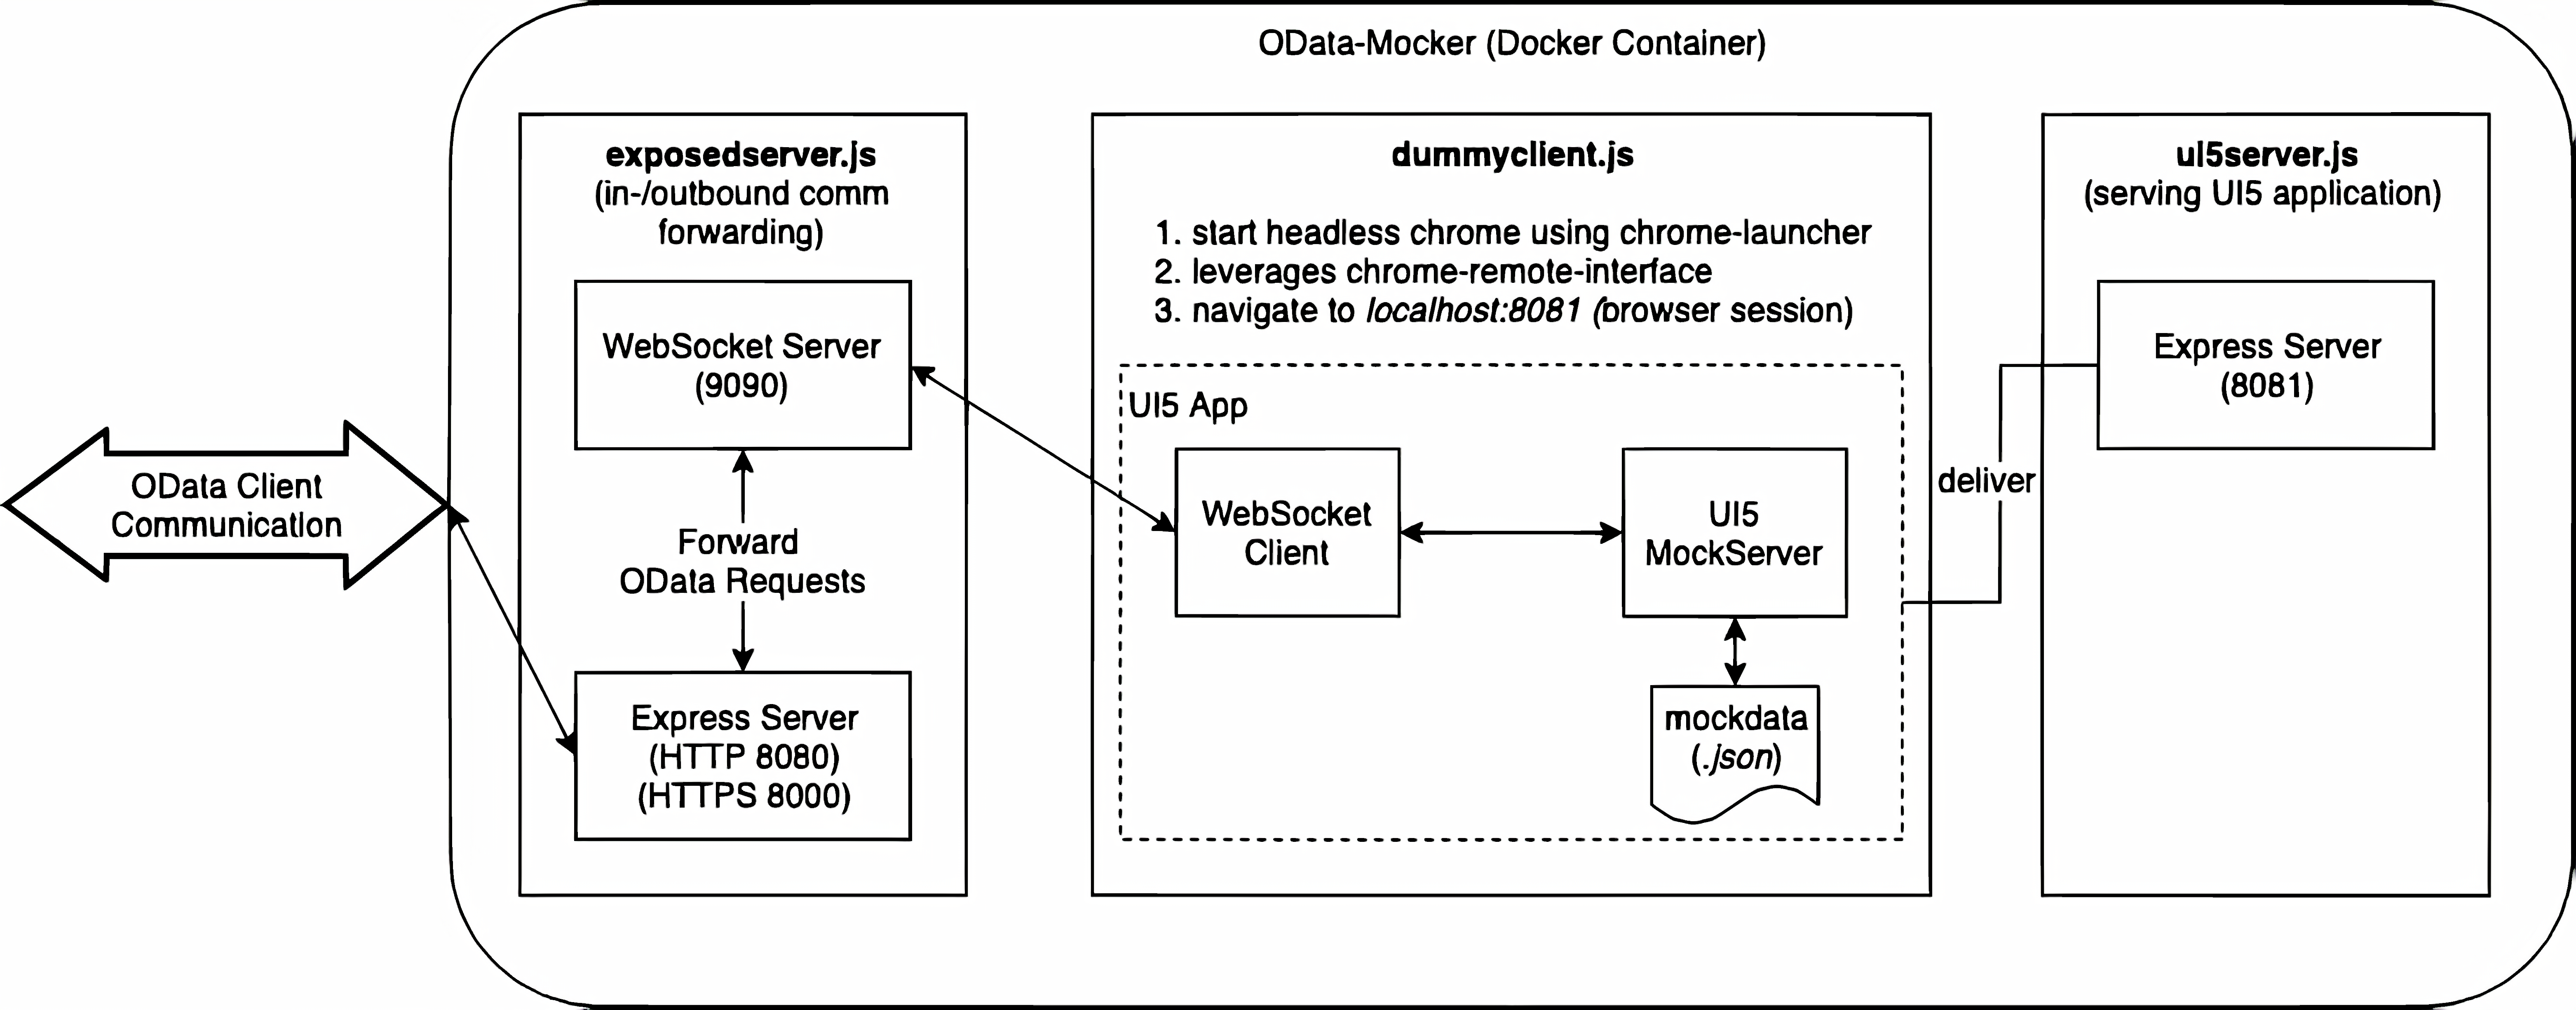
\includegraphics[width=\textwidth]{Bilder/ewm-sim_v1_4x.pdf}
    \caption{Aufbau des ewm-sim v1}
    \label{fig:ewm-sim-v1}
\end{figure}